\documentclass[aspectratio=169]{beamer}
\usetheme{Madrid}
\usecolortheme{default}

% Packages
\usepackage{graphicx}
\usepackage{booktabs}
\usepackage{amsmath}
\usepackage{hyperref}
\usepackage{tikz}
\usepackage{xcolor}
\usepackage{array}

% Custom colors
\definecolor{iiitblue}{RGB}{0, 82, 147}
\definecolor{accentorange}{RGB}{230, 126, 34}
\definecolor{successgreen}{RGB}{39, 174, 96}

\setbeamercolor{structure}{fg=iiitblue}
\setbeamercolor{title}{fg=white,bg=iiitblue}
\setbeamercolor{frametitle}{fg=white,bg=iiitblue}
\setbeamercolor{block title}{fg=white,bg=iiitblue}
\setbeamercolor{block body}{bg=iiitblue!10}

% Remove navigation symbols
\setbeamertemplate{navigation symbols}{}

% Add frame numbers
\setbeamertemplate{footline}[frame number]

% Title information
\title[Deep Retinex + DIP]{Deep Retinex Decomposition Enhanced with\\Traditional Digital Image Processing}
\subtitle{Low-Light Image Enhancement}
\author[Choudhary \& Lakhanpal]{Archit Choudhary \and Yajat Lakhanpal}
\institute[IIIT-H]{International Institute of Information Technology, Hyderabad}
\date{December 2025}

\begin{document}

%===============================================================================
% SLIDE 1: Title Slide (~30 seconds)
%===============================================================================
\begin{frame}
\titlepage
\vspace{-1cm}
\centering
\small GitHub: \url{https://github.com/firearc7/Deep-Retinex-Decomposition-Extension}
\end{frame}

%===============================================================================
% SLIDE 2: Motivation (~45 seconds)
%===============================================================================
\begin{frame}{Why Low-Light Enhancement Matters}
\begin{columns}
\begin{column}{0.5\textwidth}
\textbf{The Problem:}
\begin{itemize}
    \item Low-light conditions degrade image quality
    \item Reduced contrast and suppressed colors
    \item Increased noise levels
    \item Impacts critical applications
\end{itemize}

\vspace{0.5cm}
\textbf{Applications:}
\begin{itemize}
    \item Surveillance systems
    \item Autonomous vehicles
    \item Medical imaging
    \item Consumer photography
\end{itemize}
\end{column}
\begin{column}{0.5\textwidth}
\centering
\includegraphics[width=0.9\linewidth]{comparison_low00690.png}
\end{column}
\end{columns}
\end{frame}

%===============================================================================
% SLIDE 3: Problem with Existing Methods (~45 seconds)
%===============================================================================
\begin{frame}{Limitations of Existing Approaches}
\begin{columns}
\begin{column}{0.5\textwidth}
\textbf{Traditional Methods:}
\begin{itemize}
    \item Histogram Equalization $\rightarrow$ Unnatural results
    \item SSR/MSR $\rightarrow$ Complex tuning, halo artifacts
    \item LIME $\rightarrow$ Limited adaptability
\end{itemize}

\vspace{0.3cm}
\textbf{Deep Learning Methods:}
\begin{itemize}
    \item RetinexNet $\rightarrow$ Color artifacts
    \item EnlightenGAN $\rightarrow$ Inconsistent enhancement
    \item Zero-DCE $\rightarrow$ Over/under enhancement
\end{itemize}
\end{column}
\begin{column}{0.5\textwidth}
\begin{block}{Key Insight}
\centering
\textbf{Neither approach alone is sufficient!}
\vspace{0.3cm}

Deep learning: Good at learning patterns\\
Traditional DIP: Good at fine-grained control

\vspace{0.3cm}
$\Downarrow$
\vspace{0.3cm}

\textbf{Hybrid Approach}\\
``Train Once, Experiment Forever''
\end{block}
\end{column}
\end{columns}
\end{frame}

%===============================================================================
% SLIDE 4: Our Approach - Overview (~45 seconds)
%===============================================================================
\begin{frame}{Our Approach: Hybrid Framework}
\centering
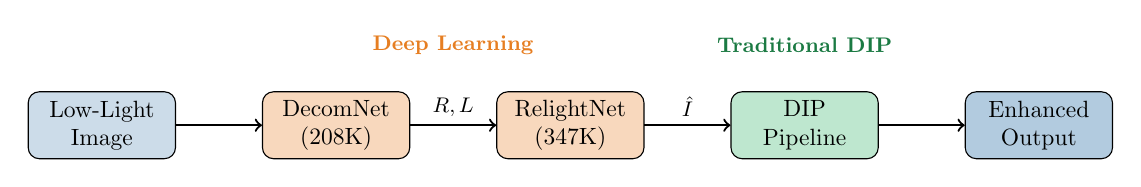
\begin{tikzpicture}[scale=0.85, transform shape,
    box/.style={draw, rounded corners, minimum width=2.2cm, minimum height=1cm, align=center}]
    % Boxes
    \node[box, fill=iiitblue!20] (input) at (0,0) {Low-Light\\Image};
    \node[box, fill=accentorange!30] (decom) at (3.5,0) {DecomNet\\(208K)};
    \node[box, fill=accentorange!30] (relight) at (7,0) {RelightNet\\(347K)};
    \node[box, fill=successgreen!30] (dip) at (10.5,0) {DIP\\Pipeline};
    \node[box, fill=iiitblue!30] (output) at (14,0) {Enhanced\\Output};
    
    % Arrows
    \draw[->, thick] (input) -- (decom);
    \draw[->, thick] (decom) -- (relight) node[midway, above] {\small $R, L$};
    \draw[->, thick] (relight) -- (dip) node[midway, above] {\small $\hat{I}$};
    \draw[->, thick] (dip) -- (output);
    
    % Labels
    \node[text=accentorange] at (5.25,1.2) {\small\textbf{Deep Learning}};
    \node[text=successgreen!70!black] at (10.5,1.2) {\small\textbf{Traditional DIP}};
\end{tikzpicture}

\vspace{0.5cm}
\begin{columns}
\begin{column}{0.33\textwidth}
\centering
\textbf{RetinexNet}\\
\small 555K params (208K + 347K)\\
Learns decomposition
\end{column}
\begin{column}{0.33\textwidth}
\centering
\textbf{DIP Techniques}\\
\small 3-stage pipeline\\
Controllable enhancement
\end{column}
\begin{column}{0.33\textwidth}
\centering
\textbf{4 Presets}\\
\small Quality/speed trade-off\\
No retraining needed
\end{column}
\end{columns}
\end{frame}

%===============================================================================
% SLIDE 5: Retinex Theory (~45 seconds)
%===============================================================================
\begin{frame}{Retinex Decomposition}
\begin{columns}
\begin{column}{0.5\textwidth}
\textbf{Retinex Theory (Land \& McCann, 1971):}
\begin{equation*}
I = R \circ L
\end{equation*}
where:
\begin{itemize}
    \item $I$ = Observed image
    \item $R$ = Reflectance (intrinsic)
    \item $L$ = Illumination (lighting)
\end{itemize}

\vspace{0.3cm}
\textbf{Enhancement:}
\begin{equation*}
\hat{I} = R \circ \hat{L}
\end{equation*}
\end{column}
\begin{column}{0.5\textwidth}
\textbf{Loss Functions:}

\textit{Reconstruction:}
\begin{equation*}
\mathcal{L}_{recon} = \|R \circ \hat{L} - I_{gt}\|_1
\end{equation*}

\textit{Smoothness:}
\begin{equation*}
\mathcal{L}_{smooth} = \sum_i \|\nabla L_i\|_1 \cdot e^{-\lambda \|\nabla R_i\|}
\end{equation*}

\textit{Total:}
\begin{equation*}
\mathcal{L} = \mathcal{L}_{recon} + \lambda_1 \mathcal{L}_{smooth} + \lambda_2 \mathcal{L}_{mutual}
\end{equation*}
\end{column}
\end{columns}
\end{frame}

%===============================================================================
% SLIDE 6: Three-Stage DIP Pipeline (~1 minute)
%===============================================================================
\begin{frame}{Three-Stage DIP Enhancement Pipeline}
\begin{columns}
\begin{column}{0.55\textwidth}
\textbf{Stage 1: Illumination Enhancement} (Primary)
\begin{itemize}
    \item \textcolor{iiitblue}{\textbf{CLAHE}}: Adaptive contrast, clip=2.0
    \item \textcolor{iiitblue}{\textbf{Bilateral Filter}}: Edge-preserving smoothing
    \item \textcolor{iiitblue}{\textbf{Adaptive Gamma}}: Content-aware brightness
    \item \textcolor{iiitblue}{\textbf{Guided Filter}}: O(N) complexity
    \item \textcolor{iiitblue}{\textbf{Multi-Scale Retinex}}: $\sigma \in \{15,80,250\}$
\end{itemize}

\vspace{0.2cm}
\textbf{Stage 2: Reflectance} (Skip---already good)

\vspace{0.2cm}
\textbf{Stage 3: Output Enhancement}
\begin{itemize}
    \item Unsharp Mask, Color Balance
    \item Local Contrast, Tone Mapping
\end{itemize}
\end{column}
\begin{column}{0.45\textwidth}
\centering
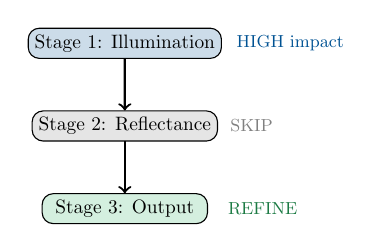
\begin{tikzpicture}[scale=0.7, transform shape]
    \node[draw, fill=iiitblue!20, rounded corners, minimum width=3cm] (s1) at (0,3) {Stage 1: Illumination};
    \node[draw, fill=gray!20, rounded corners, minimum width=3cm] (s2) at (0,1.5) {Stage 2: Reflectance};
    \node[draw, fill=successgreen!20, rounded corners, minimum width=3cm] (s3) at (0,0) {Stage 3: Output};
    
    \draw[->, thick] (s1) -- (s2);
    \draw[->, thick] (s2) -- (s3);
    
    \node[text=iiitblue] at (3,3) {\small HIGH impact};
    \node[text=gray] at (2.3,1.5) {\small SKIP};
    \node[text=successgreen!70!black] at (2.5,0) {\small REFINE};
\end{tikzpicture}

\vspace{0.5cm}
\textbf{Key Design Decision:}\\
\small Illumination $>$ Reflectance\\
(RetinexNet R is already good)
\end{column}
\end{columns}
\end{frame}

%===============================================================================
% SLIDE 7: DIP Techniques Details (~1 minute)
%===============================================================================
\begin{frame}{DIP Techniques: Mathematical Formulations}
\begin{columns}
\begin{column}{0.5\textwidth}
\textbf{1. CLAHE} (Contrast Limited Adaptive HE)
\begin{itemize}\setlength{\itemsep}{0pt}
    \item Applied to L channel in LAB space
    \item clip\_limit=2.0, tile\_grid=8$\times$8
\end{itemize}

\textbf{2. Bilateral Filter}
\begin{equation*}
I_{bf}(x) = \frac{1}{W} \sum_{x_i} I(x_i) \cdot G_s \cdot G_r
\end{equation*}
\vspace{-0.3cm}
\begin{itemize}\setlength{\itemsep}{0pt}
    \item $G_s$: Spatial, $G_r$: Range Gaussian
\end{itemize}

\textbf{3. Adaptive Gamma}
\begin{equation*}
\gamma = -0.3/\log_{10}(\mu), \quad I_{out} = I_{in}^{1/\gamma}
\end{equation*}
\end{column}
\begin{column}{0.5\textwidth}
\textbf{4. Unsharp Masking}
\begin{equation*}
I_{sharp} = I + \alpha(I - G_\sigma * I)
\end{equation*}
\vspace{-0.3cm}
\begin{itemize}\setlength{\itemsep}{0pt}
    \item $\alpha=1.2$ (balanced), $\sigma=1.0$ for edge enhancement
\end{itemize}

\textbf{5. White Balance (Gray World)}
\begin{equation*}
I_c = I_c \times \frac{\bar{I}_{gray}}{\bar{I}_c}
\end{equation*}

\textbf{6. Multi-Scale Retinex}
\begin{equation*}
MSR = \sum_{\sigma} w_\sigma \cdot [\log I - \log(G_\sigma * I)]
\end{equation*}
\vspace{-0.3cm}
\begin{itemize}\setlength{\itemsep}{0pt}
    \item $\sigma \in \{15, 80, 250\}$
\end{itemize}
\end{column}
\end{columns}
\end{frame}

%===============================================================================
% SLIDE 8: Additional DIP Techniques (~45 seconds)
%===============================================================================
\begin{frame}{Additional DIP Techniques Available}
\begin{columns}
\begin{column}{0.5\textwidth}
\textbf{Illumination Techniques:}
\begin{itemize}
    \item Histogram Equalization
    \item Multi-Scale Retinex
    \item Tone Mapping (Reinhard)
    \item Anisotropic Diffusion
    \item Guided Filtering
\end{itemize}

\vspace{0.3cm}
\textbf{Output Techniques:}
\begin{itemize}
    \item Local Contrast Enhancement
    \item Multi-Scale Detail (Laplacian)
    \item Shadow Enhancement
    \item Contrast Stretching
\end{itemize}
\end{column}
\begin{column}{0.5\textwidth}
\textbf{Edge-Preserving Smoothing:}

\small
\begin{tabular}{@{}ll@{}}
\toprule
Technique & Complexity \\
\midrule
Bilateral Filter & $O(N \cdot r^2)$ \\
Guided Filter & $O(N)$ \\
Anisotropic Diff. & $O(N \cdot k)$ \\
Domain Transform & $O(N)$ \\
\bottomrule
\end{tabular}

\vspace{0.5cm}
\textbf{Key Point:}\\
\small All techniques implemented and available for experimentation via preset configuration.
\end{column}
\end{columns}
\end{frame}

%===============================================================================
% SLIDE 9: Enhancement Presets (~30 seconds)
%===============================================================================
\begin{frame}{Enhancement Presets}
\begin{columns}
\begin{column}{0.55\textwidth}
\centering
\begin{table}
\small
\begin{tabular}{@{}lcccc@{}}
\toprule
Parameter & None & Min & \textbf{Bal} & Agg \\
\midrule
CLAHE Clip & -- & -- & \textbf{2.0} & 3.0 \\
Bilateral $d$ & -- & -- & \textbf{7} & 9 \\
Bilateral $\sigma$ & -- & -- & \textbf{50} & 75 \\
Unsharp Amt & -- & -- & \textbf{1.2} & 2.0 \\
\midrule
Time (s) & 0.005 & 0.011 & \textbf{0.089} & 0.134 \\
\bottomrule
\end{tabular}
\end{table}
\end{column}
\begin{column}{0.45\textwidth}
\textbf{Preset Use Cases:}

\vspace{0.3cm}
\textbf{None}: Raw model output\\
\small Benchmark comparison

\vspace{0.2cm}
\textbf{Minimal}: Subtle improvement\\
\small Real-time video, mobile

\vspace{0.2cm}
\textbf{Balanced} (Best): Best quality/speed\\
\small Production default

\vspace{0.2cm}
\textbf{Aggressive}: Maximum enhancement\\
\small Extremely poor inputs
\end{column}
\end{columns}
\end{frame}

%===============================================================================
% SLIDE 10: Training Details (~30 seconds)
%===============================================================================
\begin{frame}{Training Configuration}
\begin{columns}
\begin{column}{0.5\textwidth}
\textbf{Dataset: LOL (Low-Light)}
\begin{itemize}
    \item 689 training pairs
    \item 100 validation pairs
    \item Resolution: 400 $\times$ 600
    \item Paired low/normal-light images
\end{itemize}

\vspace{0.3cm}
\textbf{Training Setup:}
\begin{itemize}
    \item Epochs: 100 (best at epoch 84)
    \item Batch size: 16, Patch size: 48
    \item Optimizer: Adam ($\beta_1=0.9$, $\beta_2=0.999$)
    \item LR: $10^{-3}$ with step decay at epoch 50
    \item Training time: $\sim$18 minutes
\end{itemize}
\end{column}
\begin{column}{0.5\textwidth}
\centering
\includegraphics[width=\linewidth]{training_analysis.png}
\vspace{0.2cm}

\textbf{Best Val Loss: 0.1640}\\
\textbf{Train Loss Reduction: 59.9\%}\\
\textbf{Val Loss Reduction: 35.1\%}
\end{column}
\end{columns}
\end{frame}

%===============================================================================
% SLIDE 11: Evaluation Metrics (~30 seconds)
%===============================================================================
\begin{frame}{Evaluation Metrics (8 Metrics)}
\begin{columns}
\begin{column}{0.5\textwidth}
\textbf{No-Reference Metrics:}

\textbf{1. Entropy}: $H = -\sum p(x_i) \log_2 p(x_i)$
\begin{itemize}
    \item Information content
    \item Optimal: 7.5-8.0
\end{itemize}

\textbf{2. Contrast}: $\sigma(L)$
\begin{itemize}
    \item Standard deviation of luminance
    \item Higher = better separation
\end{itemize}

\textbf{3. Sharpness}: $\sum|G_x|^2 + |G_y|^2$
\begin{itemize}
    \item Sobel gradient magnitude
    \item Edge strength indicator
\end{itemize}

\textbf{4. Colorfulness}: Hasler-Süsstrunk
\begin{itemize}
    \item Perceptual color vividness
\end{itemize}
\end{column}
\begin{column}{0.5\textwidth}
\textbf{5. Brightness}: Mean luminance
\begin{itemize}
    \item ITU-R BT.601 weights
    \item Optimal: 0.4-0.6
\end{itemize}

\vspace{0.3cm}
\textbf{Reference-Based:}

\textbf{6. PSNR}: $20\log_{10}(MAX/\sqrt{MSE})$
\begin{itemize}
    \item Standard benchmark
\end{itemize}

\textbf{7. SSIM}: Luminance + Contrast + Structure
\begin{itemize}
    \item Better perceptual correlation
\end{itemize}

\vspace{0.3cm}
\textbf{Practical:}

\textbf{8. Processing Time}
\begin{itemize}
    \item Real-time constraint
\end{itemize}
\end{column}
\end{columns}
\end{frame}

%===============================================================================
% SLIDE 12: Quantitative Results (~1 minute)
%===============================================================================
\begin{frame}{Quantitative Results (100 Test Images)}
\begin{columns}
\begin{column}{0.5\textwidth}
\centering
\begin{table}
\small
\begin{tabular}{@{}lcccc@{}}
\toprule
Preset & Ent. & Cont. & Color. & Time \\
\midrule
Baseline & 5.91 & 23.37 & 25.05 & 0.005 \\
Minimal & 6.04 & 25.53 & 27.47 & 0.011 \\
\textbf{Balanced} & \textbf{7.32} & \textbf{57.22} & \textbf{51.20} & 0.089 \\
Aggressive & 4.60 & 63.82 & 49.36 & 0.134 \\
\midrule
Illum Only & 6.22 & 26.40 & 28.16 & 0.043 \\
Output Only & 7.17 & 56.57 & 50.49 & 0.071 \\
\bottomrule
\end{tabular}
\end{table}

\vspace{0.3cm}
\textbf{Balanced Improvements:}
\begin{itemize}
    \item Entropy: \textcolor{successgreen}{\textbf{+23.9\%}}
    \item Contrast: \textcolor{successgreen}{\textbf{+144.8\%}}
    \item Colorfulness: \textcolor{successgreen}{\textbf{+104.4\%}}
    \item Sharpness: \textcolor{successgreen}{\textbf{+1272\%}}
\end{itemize}
\end{column}
\begin{column}{0.5\textwidth}
\centering
\includegraphics[width=\linewidth]{metrics_comparison.png}
\end{column}
\end{columns}
\end{frame}

%===============================================================================
% SLIDE 13: Ablation Study (~1 minute)
%===============================================================================
\begin{frame}{Ablation Study: Why Balanced Works Best}
\begin{columns}
\begin{column}{0.42\textwidth}
\centering
\includegraphics[width=\linewidth]{ablation_study.png}
\end{column}
\begin{column}{0.58\textwidth}
\small
\textbf{1. Information Preservation}
\begin{itemize}\setlength{\itemsep}{0pt}
    \item Highest entropy (7.32); Aggressive destroys tonal info (4.60)
\end{itemize}

\textbf{2. Optimal Contrast (+144.8\%)}
\begin{itemize}\setlength{\itemsep}{0pt}
    \item CLAHE + Bilateral synergy without saturation artifacts
\end{itemize}

\textbf{3. Natural Sharpness}
\begin{itemize}\setlength{\itemsep}{0pt}
    \item No halo artifacts; Aggressive causes edge overshoot
\end{itemize}

\textbf{4. Color Fidelity (+104.4\%)}
\begin{itemize}\setlength{\itemsep}{0pt}
    \item Highest colorfulness (51.20) with natural relationships
\end{itemize}

\textbf{5. Appropriate Brightness}
\begin{itemize}\setlength{\itemsep}{0pt}
    \item Preserves highlight headroom
\end{itemize}
\end{column}
\end{columns}
\end{frame}

%===============================================================================
% SLIDE 14: Visual Results (~45 seconds)
%===============================================================================
\begin{frame}{Visual Results}
\centering
\includegraphics[width=0.85\linewidth]{comparison_low00696.png}

\vspace{0.3cm}
\textbf{Progressive enhancement: Input $\rightarrow$ RetinexNet $\rightarrow$ DIP Pipeline $\rightarrow$ Output}
\end{frame}

%===============================================================================
% SLIDE 15: More Visual Results (~30 seconds)
%===============================================================================
\begin{frame}{More Visual Comparisons}
\centering
\includegraphics[width=0.85\linewidth]{comparison_low00690.png}

\vspace{0.3cm}
Natural-looking enhancement with improved visibility, enhanced colors, and preserved details
\end{frame}

%===============================================================================
% SLIDE 16: Demo Slide
%===============================================================================
\begin{frame}
\centering
\vspace{2cm}
{\Huge \textbf{DEMO}}

\vspace{1cm}
{\Large Live demonstration of the enhancement system}

\vspace{1cm}
\begin{itemize}
    \centering
    \item[$\bullet$] Custom image enhancement
    \item[$\bullet$] Preset comparison (None vs Balanced vs Aggressive)
    \item[$\bullet$] Real-time processing
\end{itemize}
\end{frame}

%===============================================================================
% SLIDE 17: Design Decisions (~30 seconds)
%===============================================================================
\begin{frame}{Key Design Decisions}
\begin{columns}
\begin{column}{0.5\textwidth}
\textbf{Why CLAHE on Illumination?}
\begin{itemize}
    \item Illumination is smooth (no texture)
    \item CLAHE won't amplify texture noise
    \item Output has reflectance texture
\end{itemize}

\vspace{0.3cm}
\textbf{Why Skip Reflectance?}
\begin{itemize}
    \item RetinexNet R is already high quality
    \item No consistent improvement observed
    \item Risk of color shifts
\end{itemize}

\vspace{0.3cm}
\textbf{Why Post-Processing?}
\begin{itemize}
    \item No retraining needed
    \item 100+ configurations instantly
    \item Flexibility $>$ Optimality
\end{itemize}
\end{column}
\begin{column}{0.5\textwidth}
\textbf{Stage Separation Results:}

\vspace{0.3cm}
\begin{tabular}{@{}lc@{}}
\toprule
Configuration & Sharpness \\
\midrule
Baseline & 150.84 \\
Illumination Only & 186.31 (+23.5\%) \\
Output Only & 2370.22 (+1471\%) \\
Balanced (both) & 2069.40 (+1272\%) \\
\bottomrule
\end{tabular}

\vspace{0.5cm}
\textbf{Key Insight:}\\
Output enhancement amplifies illumination improvements
\end{column}
\end{columns}
\end{frame}

%===============================================================================
% SLIDE 18: Comparison with SOTA (~30 seconds)
%===============================================================================
\begin{frame}{Advantages Over Existing Methods}
\begin{columns}
\begin{column}{0.33\textwidth}
\begin{block}{vs. Pure Deep Learning}
\begin{itemize}
    \item Controllable parameters
    \item No retraining needed
    \item Interpretable processing
    \item Adapt to use cases
\end{itemize}
\end{block}
\end{column}
\begin{column}{0.33\textwidth}
\begin{block}{vs. Pure Traditional}
\begin{itemize}
    \item Handles complex lighting
    \item Learned decomposition
    \item More robust
    \item Better generalization
\end{itemize}
\end{block}
\end{column}
\begin{column}{0.33\textwidth}
\begin{block}{vs. Other Hybrids}
\begin{itemize}
    \item Modular architecture
    \item Independent updates
    \item Flexible presets
    \item Three-stage pipeline
\end{itemize}
\end{block}
\end{column}
\end{columns}

\vspace{0.3cm}
\centering
\begin{table}
\small
\begin{tabular}{@{}lc@{}}
\toprule
Component & Specification \\
\midrule
Total Parameters & 555,205 \\
Training Time & $\sim$18 minutes \\
Inference & Real-time capable \\
DIP Techniques & 16 implemented \\
\bottomrule
\end{tabular}
\end{table}
\end{frame}

%===============================================================================
% SLIDE 19: Future Work (~45 seconds)
%===============================================================================
\begin{frame}{Future Work}
\begin{columns}
\begin{column}{0.5\textwidth}
\textbf{Enhancement Techniques:}
\begin{itemize}
    \item Frequency domain processing
    \item Homomorphic filtering
    \item FFT-based denoising
    \item Advanced color space processing
\end{itemize}

\vspace{0.3cm}
\textbf{Content-Aware Processing:}
\begin{itemize}
    \item Adaptive preset selection
    \item Semantic segmentation-guided
    \item Automatic parameter tuning
\end{itemize}
\end{column}
\begin{column}{0.5\textwidth}
\textbf{Quality Assessment:}
\begin{itemize}
    \item NIQE, BRISQUE metrics
    \item LPIPS perceptual metric
    \item Automated optimization
\end{itemize}

\vspace{0.3cm}
\textbf{Applications:}
\begin{itemize}
    \item Video processing
    \item Temporal consistency
    \item Mobile deployment
    \item GPU acceleration
\end{itemize}
\end{column}
\end{columns}
\end{frame}

%===============================================================================
% SLIDE 20: Conclusion (~30 seconds)
%===============================================================================
\begin{frame}{Conclusion}
\begin{block}{Summary}
\begin{itemize}
    \item Proposed a \textbf{hybrid framework} combining deep Retinex decomposition with \textbf{traditional DIP techniques}
    \item \textbf{``Train Once, Experiment Forever''}: No retraining for new enhancement combinations
    \item \textbf{Three-stage pipeline}: Illumination, Reflectance (skip), Output enhancement
    \item \textbf{Balanced preset} achieves optimal results:
    \begin{itemize}
        \item +23.9\% entropy, +144.8\% contrast, +1272\% sharpness, +104.4\% colorfulness
    \end{itemize}
    \item \textbf{Key insight}: Illumination enhancement $>$ Reflectance enhancement
\end{itemize}
\end{block}

\vspace{0.2cm}
\centering
\begin{block}{Code Available}
\centering
\url{https://github.com/firearc7/Deep-Retinex-Decomposition-Extension}
\end{block}
\end{frame}

%===============================================================================
% SLIDE 21: Thank You
%===============================================================================
\begin{frame}
\centering
\vspace{1.5cm}
{\Huge \textbf{Thank You!}}

\vspace{1cm}
{\Large Questions?}

\vspace{1.5cm}
\textbf{Archit Choudhary \& Yajat Lakhanpal}\\
International Institute of Information Technology, Hyderabad

\vspace{0.5cm}
\small
GitHub: \url{https://github.com/firearc7/Deep-Retinex-Decomposition-Extension}
\end{frame}

\end{document}
